\documentclass[10pt]{article}
\usepackage[letterpaper]{geometry}
\usepackage{listings}
\usepackage{graphicx}
\renewcommand{\figurename}{Imagen}


\title{\textbf{Reporte: Creación de Estructuras con una Calculadora}}
\author{Diego Ruiz Mora | 2202000335}
\date{13-Septiembre-2023}

\begin{document}
	
	\maketitle
	\section{Primera Estructura}
	Para generar la estructura de la \emph{imagen \ref{fig:est1}} tendremos que hacer un pequeño cambio al código donde tendremos que generar solamente un hijo en el código de calculadora y quitar la condición en la que se hacia la petición de una operación a ejecutar. Esto se ve en la \emph{imagen \ref{fig:calculadora}}, que después de la creación del hijo con la instrucción \textbf{idf=fork()}, al hijo le asignamos el nuevo código que en este caso será el de el proceso \emph{suma} como lo hicimos en la tarea, solamente que solo se creará a un hijo en este caso. 
	\\\\
	Por otro lado, para el caso de los procesos hijos es algo parecido, en general notaremos que es la misma modificación para el resto de los códigos, donde buscaremos que cada uno de los procesos tenga un hijo, al que le asignara el código del siguiente proceso, ese siguiente proceso creará un hijo y a su vez le dará el código respectivo del siguiente, así de manera simultanea. 
	\begin{figure}[h!]
		\centering
		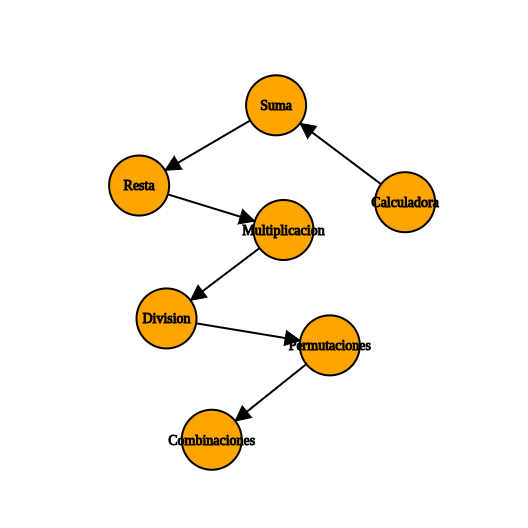
\includegraphics[width=0.5\linewidth]{graph.png}
		\caption{Estructura}
		\label{fig:est1}
	\end{figure}
	\begin{figure}[h!]
		\centering
		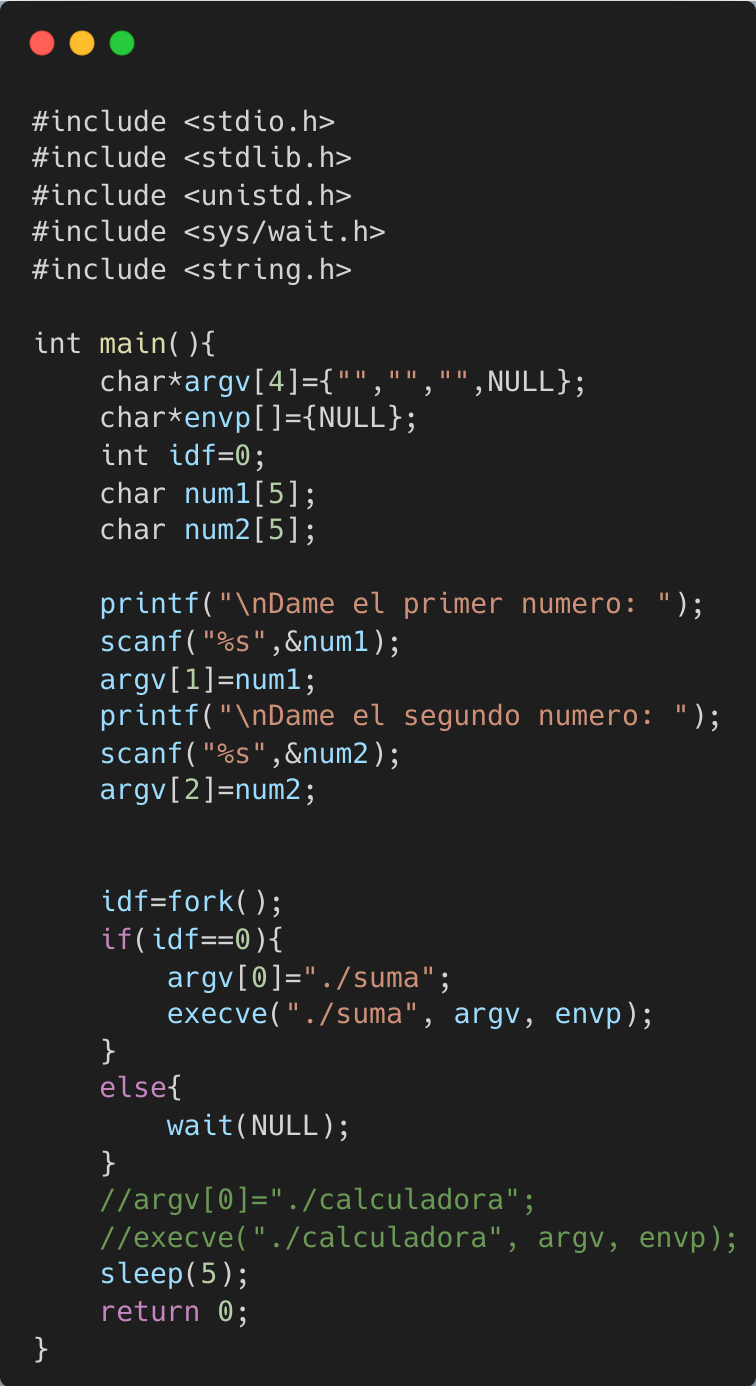
\includegraphics[width=0.4\linewidth]{calculadora.png}
		\caption{Código de calculadora.c}
		\label{fig:calculadora}
	\end{figure}
	\newpage
	Para ver de manera más fiel de lo que hablamos, tendremos que recurrir a la \emph{imagen \ref{fig:suma}}, donde veremos el código respectivo para la \emph{suma} y como es que creamos un hijo y después le asignamos a este hijo el código de la siguiente operación. 
	\\\\
	Y como bien dijimos esto se repetirá hasta que se llegue al último proceso que es \emph{combinaciones} que es el que no se verá modificado en su código. También es importante denotar que en los demás códigos incorporemos una instrucción \textbf{wait(NULL)} que nos permitirá esperar a que los procesos hijos dejen de ejecutar para que los procesos padres terminen. Esto nos permitirá visualizar el árbol de procesos. 
	\begin{figure}[h!]
		\centering
		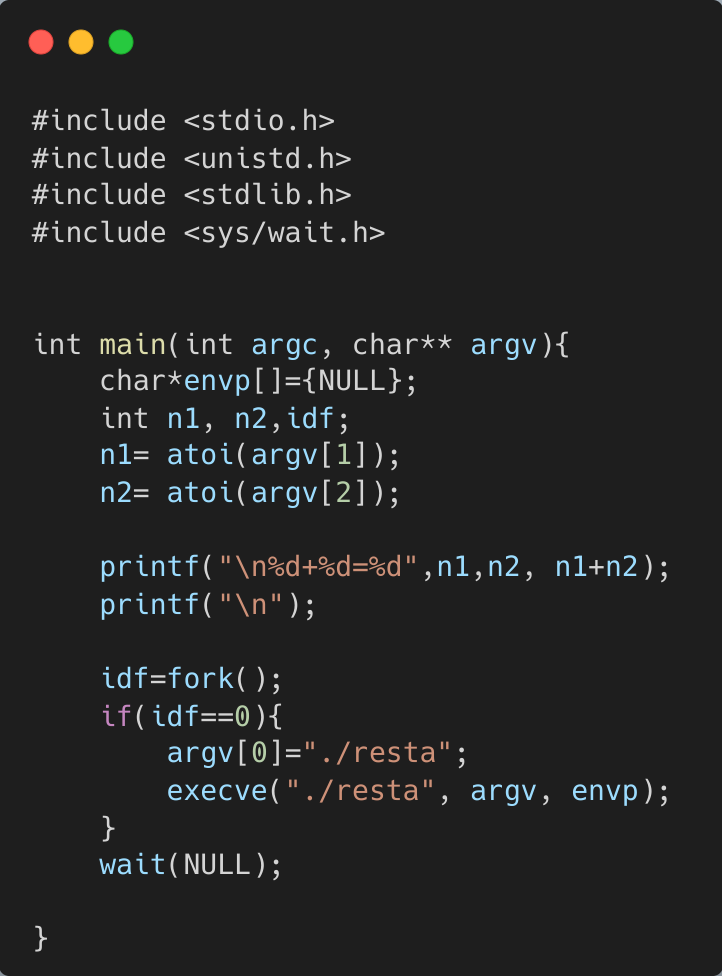
\includegraphics[width=0.4\linewidth]{suma.png}
		\caption{Código de suma.c}
		\label{fig:suma}
	\end{figure}
	\\\\
	Veremos en la \emph{imagen \ref{fig:pruebae1}} que es correcta esta forma de realizar el código ya que la estructura generada es la deseada, donde cada uno de los procesos tiene un hijo que es el siguiente proceso a ejecutar. De igual forma al ver el código ejecutado notaremos que los valores que pasan son los mismo, ya que esto no se modificó, aunque si se podría lograr modificando el vector de argumentos en cada proceso antes de asignar el código al siguiente hijo. 
	\begin{figure}[h!]
		\centering
		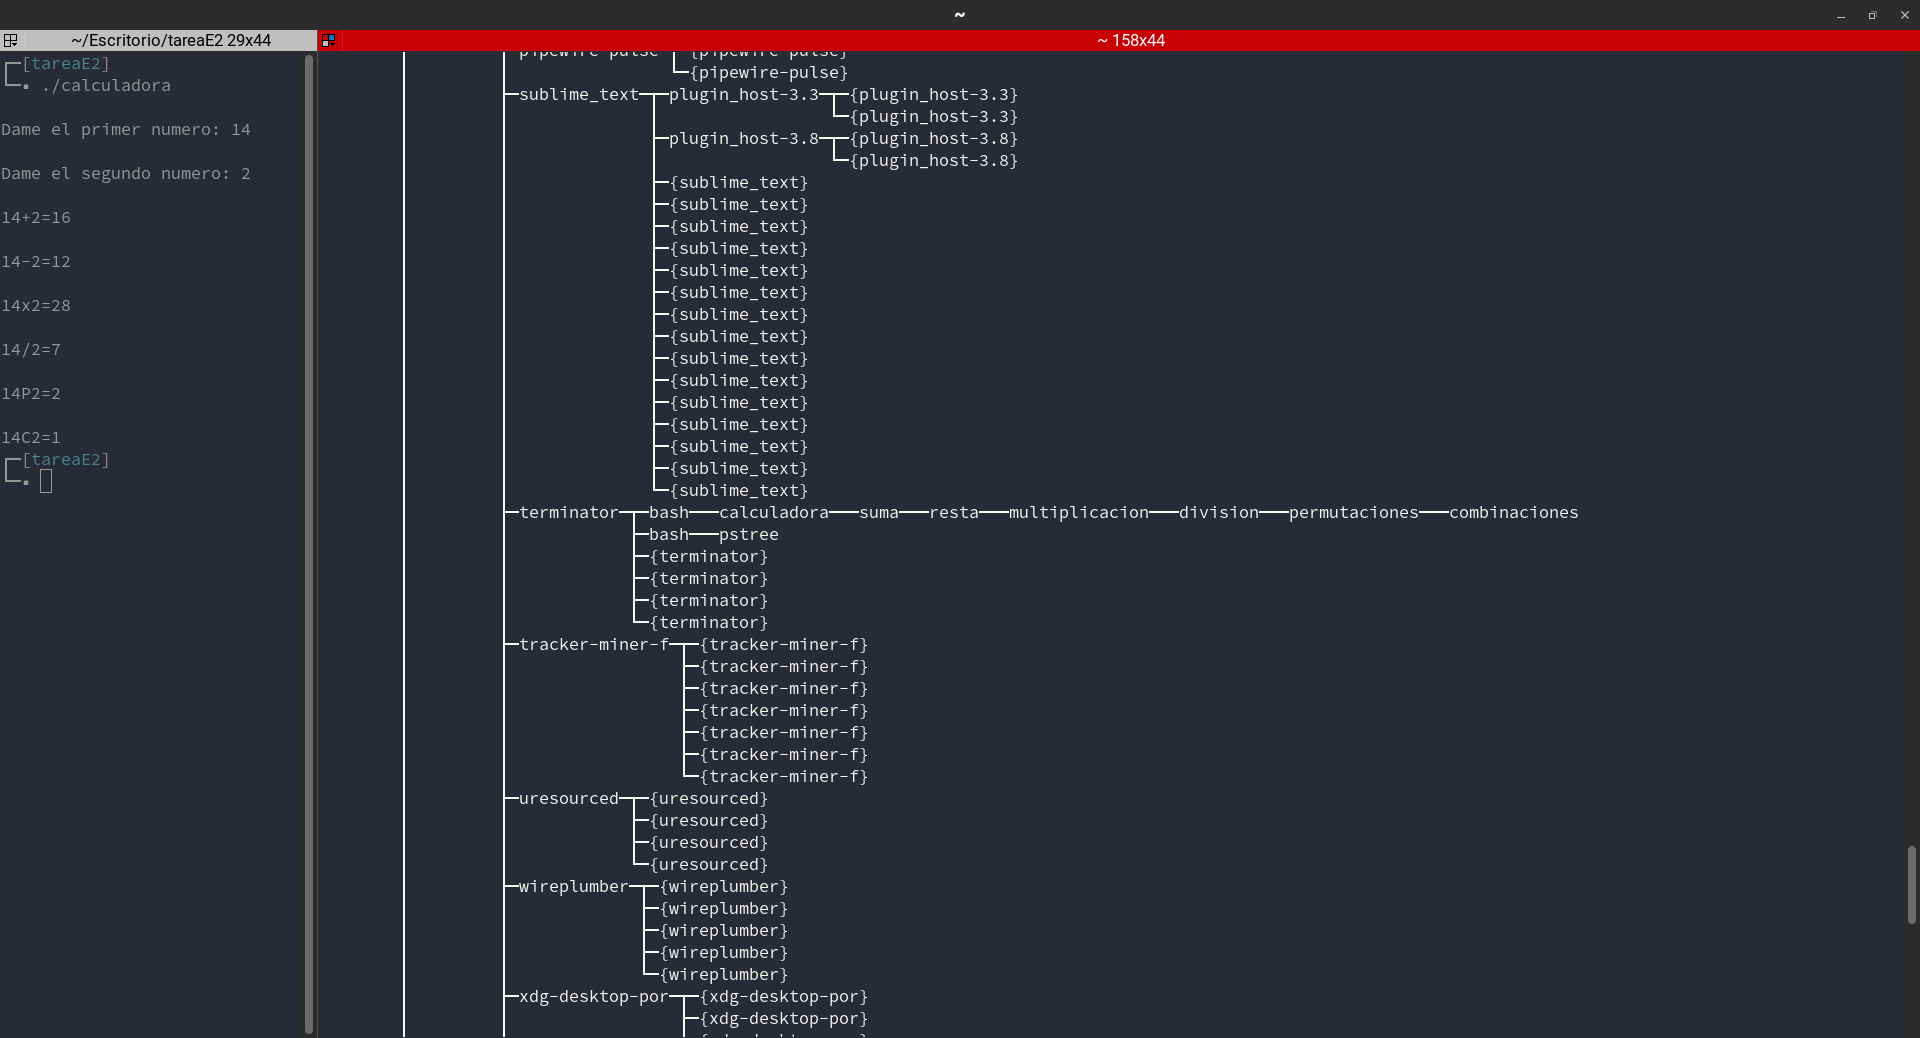
\includegraphics[width=\linewidth]{pruebaE1}
		\caption{Estructura generada}
		\label{fig:pruebae1}
	\end{figure}
	\newpage
	
	\section{Segunda Estructura}
	Para realizar la siguiente estructura mostrada en \emph{imagen  \ref{fig:est2}} modificaremos solamente  el código de \emph{calculadora} ya que es el único que genera hijos, de hecho la estructura es muy parecida a lo que se llamaría un \textit{abanico}. 
	\begin{figure}[h!]
		\centering
		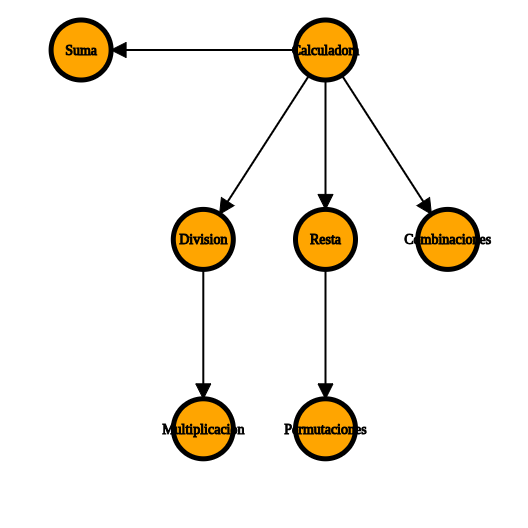
\includegraphics[width=0.5\linewidth]{graph2.png}
		\caption{Estructura}
		\label{fig:est2}
	\end{figure}
	\\
	Revisaremos el código de la \emph{imagen \ref{fig:calculadora2}}, respectivo a \textit{calculadora} , donde encontraremos seis instrucciones \textbf{fork()}, cada una asignada a un identificador diferente para no tener problemas al momento de crear cada uno de los hijos, claro que pudimos ahorrarnos algunas, pero es más sencillo de esta forma. 
	\\\\
	Dentro de cada una de las instrucciones encontraremos la asignación del nombre del proceso al primer elemento  del vector de argumentos, seguido encontraremos la asignación del código a este respectivo hijo generado lineas antes. Básicamente el proceso es el mismo, podríamos incluso facilitar la creación con el uso de una estructura de repetición. 
	\\\\
	Por último agregamos una instrucción \textbf{sleep()} para lograr que la ejecución tarde un poco en ejecutar y nos permita observar los resultados de la ejecución, lo cual es posible observar en la \emph{imagen \ref{fig:pruebae2}} , donde es claro que la estructura generada es la deseada. 
	\\
	Es importante ver el como se entregan los resultados en la terminal, ya que estos no se resuelven de manera ordenada debido a las condiciones de carrera, a pesar de que los procesos se hayan ejecutado con cierta lógica de orden dentro del código. 
	\begin{figure}[h!]
		\centering
		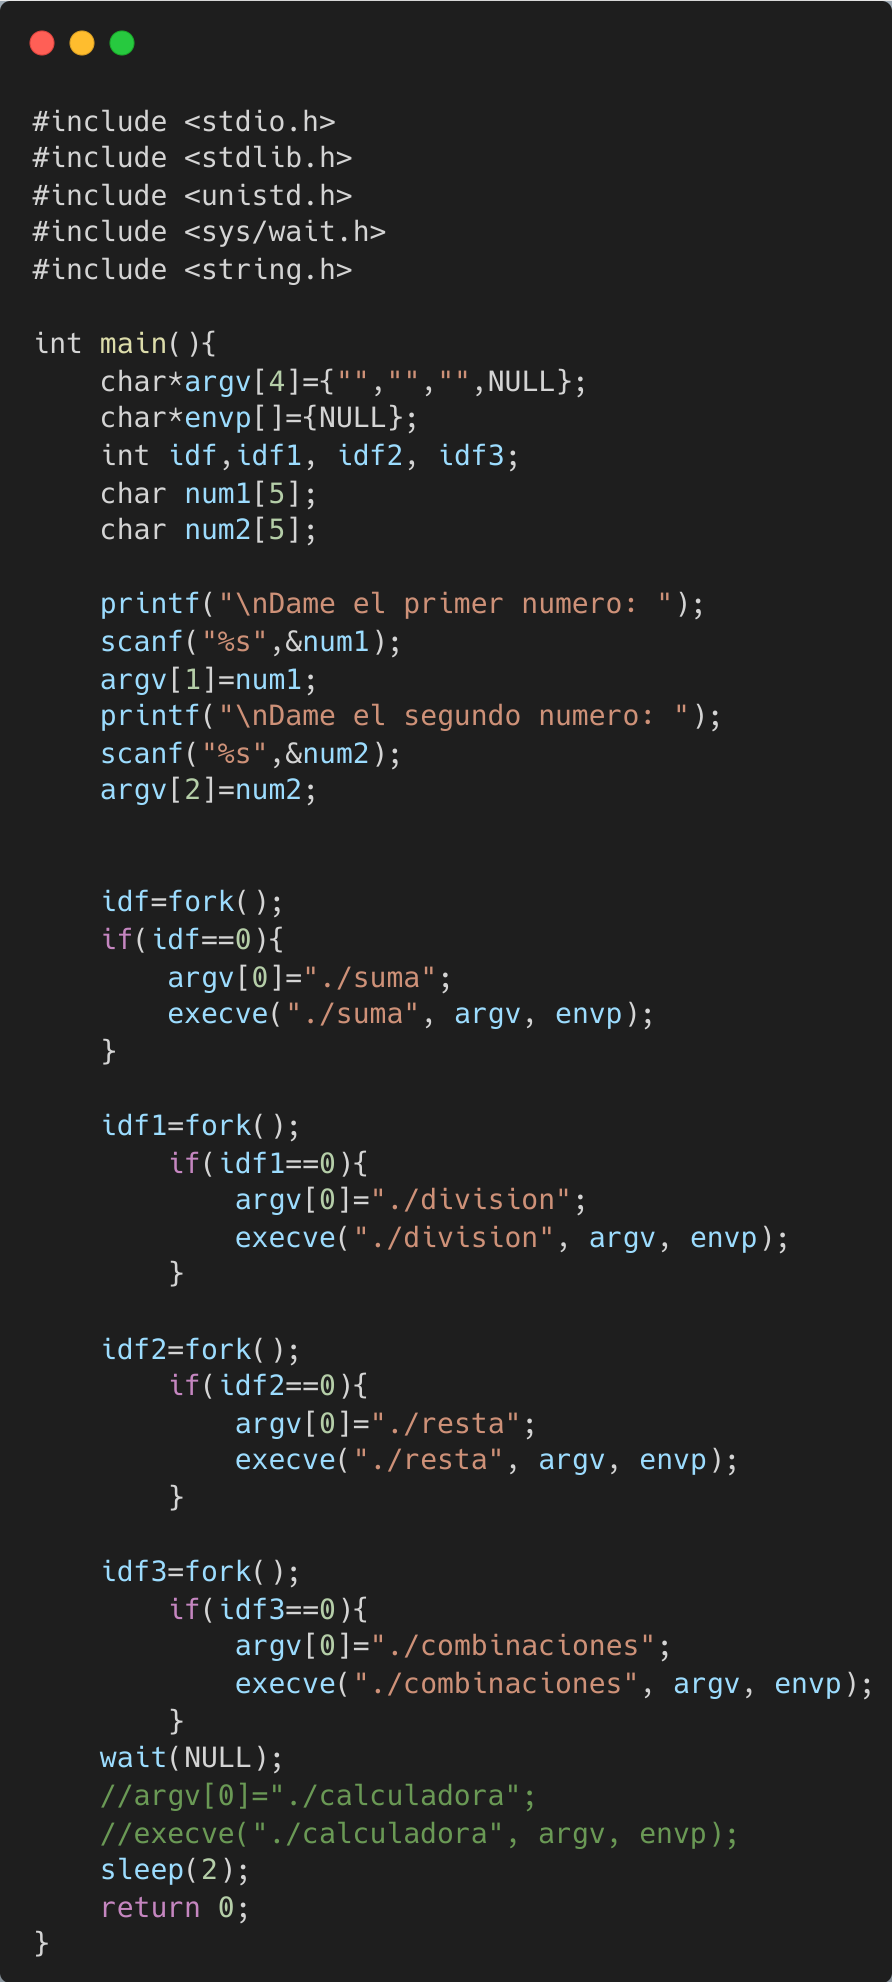
\includegraphics[width=0.5\linewidth]{calculadora2.png}
		\caption{Código calculadora.c}
		\label{fig:calculadora2}
	\end{figure}
	\begin{figure}[h!]
		\centering
		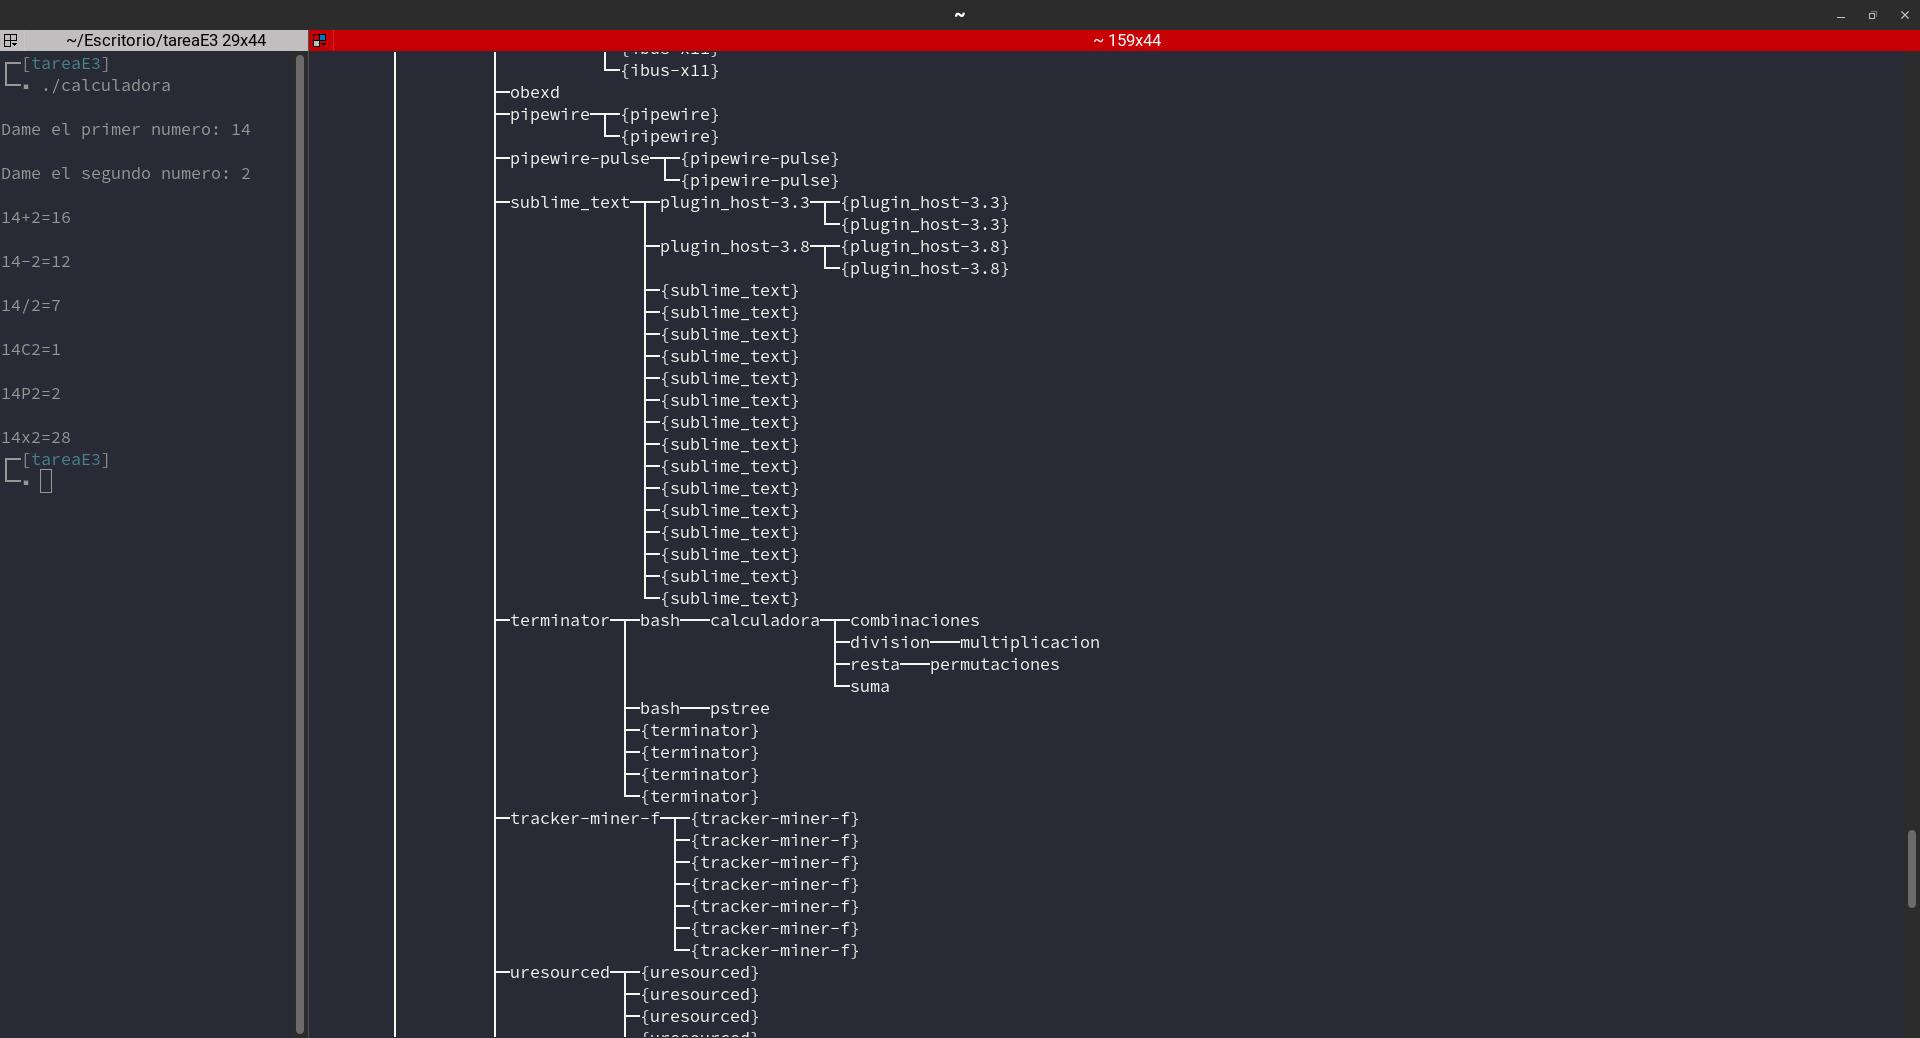
\includegraphics[width=\linewidth]{pruebaE2}
		\caption{Estructura generada}
		\label{fig:pruebae2}
	\end{figure}
	


	
	
\end{document}